In the paper~\cite{the-notion-of-dimension-in-geometry-and-algebra}, \href{http://en.wikipedia.org/wiki/Yuri_I._Manin}{Yuri I. Manin} writes:

\begin{quote}
  ``This guess involves the conjectural existence of a geometrical world defined over ``an absolute point''~$\Spec\mathbb{F}_1$ where~$\mathbb{F}_1$ is a mythical field with one element. For some insights about this world, see~\cite{sur-les-analogues-algebriques-des-groupes-semi-simples-complexes}, \cite{hurwitz-inequalities-for-number-fields}, \cite{letters-to-manin}, \cite{cohomology-determinants-and-reciprocity-laws}, \cite{three-dimensional-hyperbolic-geometry}, \cite{les-varietes-sur-le-corps-a-un-element}.''
\end{quote}

The first of two letters from \href{http://www.pdmi.ras.ru/eng/perso/smirnov.php}{Alexandr Smirnov} to Manin also appears in the paper~\cite{lambda-rings-and-the-field-with-one-element} by \href{http://maths.anu.edu.au/~borger/}{James Borger}:

\begin{quote}
  ``The second purpose is to prove the Riemann hypothesis. With the analogy between integers and polynomials in mind, we might hope that~$\Spec\mathbb{Z}$ would be a kind of curve over~$\Spec\mathbb{F}_1$, that~$\Spec\mathbb{Z}\times\Spec\mathbb{Z}$ would not only make sense but be a surface bearing some kind of intersection theory, and that we could then mimic over~$\mathbb{Z}$ Weil's~proof~\cite{on-the-riemann-hypothesis-in-function-fields} of the Riemann hypothesis over function fields.
  
  The origins of this idea are unknown to me. Manin~\cite{lectures-on-zeta-functions-and-motives} mentions it explicitly. According to Smirnov~\cite{letters-to-manin}, the idea occurred to him in~1985 and he mentioned it explicitly in a talk in Shafarevich's seminar in~1990. It may well be that a number of people have had the idea independently since the appearance of Weil's proof.''
\end{quote}

I thank Yuri Manin and James Borger for providing me with copies of these letters. Some of their content is crucial to understand the genesis of Smirnov's paper \cite{hurwitz-inequalities-for-number-fields}, which is the first paper we will study in the seminar.

\begin{figure}[ht!]
  \centering
  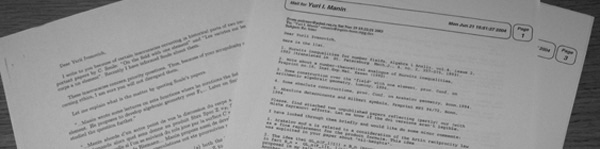
\includegraphics[width=11cm]{the-smirnov-letters/letters}
  \caption{The actual Smirnov letters}
  \label{figure:smirnov-letters}
\end{figure}

From Smirnov's letter to Yu. I. Manin, dated September 29th 2003:

\begin{quote}
  ``As to my investigations, I work on the topic since 1985. Till then the subject has been paid next to no attention, with the exception of a paper (\emph{see \cite{sur-les-analogues-algebriques-des-groupes-semi-simples-complexes}}) by \href{http://en.wikipedia.org/wiki/Jacques_Tits}{Jacques Tits} (1957) and the idea (due to \href{http://en.wikipedia.org/wiki/Daniel_Quillen}{Daniel Quillen}?) to interpret the Barrat-Priddy-Quillen theorem as the equality~$\mathrm{K}(\mathbb{F}_1)=\pi^{\mathrm{st}}(\mathrm{S}^0)$.

  My initial goal was (and still is) to construct a `world' which contains algebraic geometry as well as arithmetic, and where all constructions from algebraic geometry (including $\Spec\mathbb{Z}\times\Spec\mathbb{Z}$) would be available. From the beginning I believed that this could give an approach to the Riemann hypothesis (similar to Weil's approach).

  I started with the idea, known for me from a seminar (early 80's), that sets can be considered as vectorspaces over~$\mathbb{F}_1$. I believed that this idea was promising in view of the mentioned interpretation of the Barrat-Priddy-Quillen theorem.

  Since I couldn't invent~$\Spec\mathbb{Z}\times\Spec\mathbb{Z}$, I worked out a strategy which I have adhered:
  \begin{itemize}
    \item If we can't develop the whole desired theory, we should invent as many objects over~$\mathbb{F}_1$ as possible and establish connections between them.
    \item Since the situation is extremely rigid, any flexibility of constructions would lead to essential progress.
  \end{itemize}

  The idea to construct finite extensions of~$\mathbb{F}_1$ (thus getting the missing flexibility) and the suggestion to consider the monoids $0\cap\unityroots$ as a naive technical approximation to these extensions arose precisely from this strategy.

  Having on hand the extensions, I discovered I could effectively work with a number of new objects over~$\mathbb{F}_1$, for instance with~$\mathbb{P}^n$. Thus I decided to handle intersection theory (which is part of Weil's approach to the Riemann hypothesis) on the surface~$\mathbb{P}^1/\mathbb{F}_1\times\Spec\mathbb{Z}$ instead of the more complicated~$\Spec\mathbb{Z}\times\Spec\mathbb{Z}$. The Hurwitz genus formula for a map of curves $f\colon X\rightarrow Y$ can be viewed as an example of using intersection theory on the surface $X\times Y$, and I started with it. I succeeded in stating a certain approximation to the \href{http://en.wikipedia.org/wiki/Riemann–Hurwitz_formula}{Hurwitz formula} for the `map'~$f\colon\Spec\mathbb{Z}\to\mathbb{P}^1/\mathbb{F}_1$ where~$f\in\mathbb{Q}$.

  It was somewhat surprising (and confirming the importance of the approach) that this approximation gave very profound assertions like the \href{http://en.wikipedia.org/wiki/Abc_conjecture}{$abc$-conjecture} and others. An impulse to \href{http://matrix.cmi.ua.ac.be/ngeometry/library/Smirnov1991.pdf}{publish these results} (\emph{the unfinished and unpublished paper in~\cite{cohomology-determinants-and-reciprocity-laws}}) was given to me by \href{http://directory.math.yale.edu/public_html/People/mk486.html}{Mikhael Kapranov} after he and \href{http://en.wikipedia.org/wiki/Vladimir_Voevodsky}{Vladimir Voevodsky} learned about them (1988 or 1989)."
\end{quote} 
